%%%%%%%%%%%%%%%%%%%%%%% file typeinst.tex %%%%%%%%%%%%%%%%%%%%%%%%%
%
% This is the LaTeX source for the instructions to authors using
% the LaTeX document class 'llncs.cls' for contributions to
% the Lecture Notes in Computer Sciences series.
% http://www.springer.com/lncs       Springer Heidelberg 2006/05/04
%
% It may be used as a template for your own input - copy it
% to a new file with a new name and use it as the basis
% for your article.
%
% NB: the document class 'llncs' has its own and detailed documentation, see
% ftp://ftp.springer.de/data/pubftp/pub/tex/latex/llncs/latex2e/llncsdoc.pdf
%
%%%%%%%%%%%%%%%%%%%%%%%%%%%%%%%%%%%%%%%%%%%%%%%%%%%%%%%%%%%%%%%%%%%

%\documentclass[runningheads,a4paper]{llncs}
\documentclass[a4paper]{llncs}

%\usepackage{amssymb}
%\setcounter{tocdepth}{3}
%\usepackage{graphicx}
\usepackage{url}
\usepackage[utf8]{inputenc}
\usepackage{todonotes}
%\usepackage{hyperref}
%\usepackage{booktabs}
%\usepackage{subfig}
%\usepackage{array}
\usepackage[portuges]{babel}

% \newcommand{\papertitle}{A Distributed Computing Framework for Heterogeneous Environments}


\newcommand{\papertitle}{PCap com filtragem orientada ao processo}

%\newcommand{\papertitle}{Leveraging GPUs for Scientific Computing}

%\hypersetup{pdfborder=0 0 0,
%            pdfauthor={Nuno Martins \and Vítor Duarte},
%%            pdfcreator=,
%            pdfkeywords={Pcap, linux, monitorização,},
%%            pdfsubject=TesteSubject,
%            pdftitle={\papertitle}
%           }


\urldef{\mailsa}\path|nuno.m.g.martins@gmail.com|
\urldef{\mailsb}\path|vad@di.fct.unl.pt|    

\newcommand{\keywords}[1]{\par\addvspace\baselineskip
\noindent\keywordname\enspace\ignorespaces#1}

\newcommand{\td}[1]{\todo[inline]{#1}}


\begin{document}

\mainmatter  % start of an individual contribution

% first the title is needed
\title{\papertitle}

\author{Nuno Martins\inst{1} e Vítor Duarte\inst{2}}
%
\authorrunning{\papertitle}
% (feature abused for this document to repeat the title also on left hand pages)

% the affiliations are given next; don't give your e-mail address
% unless you accept that it will be published
\institute{\email{nuno.m.g.martins@gmail.com} \and \email{vad@di.fct.unl.pt}\\
CITI --- Departamento de Informática,\\
Faculdade de Ciências e Tecnologia,\\
Universidade Nova de Lisboa, Portugal}
%\mailsa \qquad \mailsb}

%
% NB: a more complex sample for affiliations and the mapping to the
% corresponding authors can be found in the file "llncs.dem"
% (search for the string "\mainmatter" where a contribution starts).
% "llncs.dem" accompanies the docume\label{•} nt class "llncs.cls".
%

%\toctitle{Lecture Notes in Computer Science}
%\tocauthor{Authors' Instructions}
\maketitle

\begin{abstract}

A monitorização do comportamento dos processos é uma das melhores formas de compreender a sua execução real, de detectar erros e avaliar o seu real desempenho, ainda mais se não for possível aceder ao seu código fonte. No entanto, o impacto no desempenho e comportamento das aplicações pode ser bastante significativo.
 O caso das interacções entre processos via rede não é excepção, e mesmo sistemas populares como PCap com auxílio do núcleo do sistema de operação, podem introduzir uma grande perturbação agravada pela dificuldade de obter apenas os dados que dizem respeito à aplicação sob observação.
Este trabalho estende o suporte dado no núcleo Linux a este sistema, por forma a permitir capturar as interacções via rede de processos específicos, facilitando a sua análise e procurando também limitar o impacto deste tipo de monitorização.
  Para tal, foi criada uma forma de filtragem nos \emph{lpf-filters}, usados pelo PCap que, dinamicamente, através da monitorização das chamadas ao sistema do processo, permite manter os endereços e portos em utilização pelo processo alvo e capturar apenas o seu tráfego. Deste modo é possível, sem conhecimento prévio ou alterações aos processos, obter apenas os dados relevantes. Esta extensão introduz assim, sem incompatibilidades, uma nova funcionalidade, com vantagens relativamente à perturbação do restante sistema quando se pretende analisar apenas uma determinada aplicação. 

\keywords{Instrumentação, Monitorização, KProbes, Núcleo do Linux, PCap}
\end{abstract}

\section{Introdução}
\label{sec:introduction}

A monitorização permite que diferentes partes de um programa ou processo possam ser analisados. Podemos analisar os tempos de execução de determinadas funções ou de todo o processo, é possível analisar as suas interacções com o exterior bem como outros parâmetros tais como a percentagem de utilização do(s) cpu(s) ou a utilização de memória.
%auditar, correcção, segurança, etc



%\section{Monitorização}
%\label{sec:mon_intro}

%apenas os conceitos base
%3/4 parágrafos

A monitorização causa perdas no desempenho e por isso é desejável que seja o menor possível. 
A monitorização de sistemas exige sempre a execução de acções específicas para a detecção e/ou registo dos acontecimentos que se pretendem observar que concorrem no uso dos recursos disponíveis com o próprio sistema monitorizado. O grau da perturbação introduzida no sistema monitorizado depende dos mecanismos usados, nível de detalhe, volume de dados recolhidos, etc. É comum o recurso a mecanismos de instrumentação de código para a implementação destas acções, possivelmente a diferentes níveis, como sejam o do programa, bibliotecas, ou internas ao sistema de operação.

 Quando se recorre a mecanismos de monitorização presentes nos sistemas de operação, como, por exemplo, na observação das interacções via rede, pode-se beneficiar de um mecanismo geral e eficiente, mas que ainda leva à execução de acções extra no sistema de operação (muitas vezes mais eficientes do que tentar obter a mesma funcionalidade a outro nível), mas pode ser agravado devido à cópia dos dados recolhidos no núcleo do sistema para as ferramentas que os usam e consequentes trocas de contexto (kernel-level/user-level).

A instrumentação do código pode ser efectuada de forma estática ou dinâmica. Na instrumentação estática é necessário ter acesso ao código fonte, passar pelo ciclo colocação dos pontos a analisar, compilar, executar e novamente colocação dos pontos a analisar. Desta forma não é possível modificar os pontos de instrumentação nem interagir com estes. Na instrumentação dinâmica é possível efectuar sem acesso ao código fonte, permite a colocação e remoção de pontos de instrumentação, bem como interagir com o sistema de monitorização, alguns deles, mesmo durante a execução do sistema. 

Outra forma de classificar estes sistemas tem em conta o tipo de processamento efectuado e de informação recolhida. Podemos distinguir entre os que permitem detectar eventos e obter um traço detalhado da execução e aqueles que efectuam amostragens ao estado do sistema em determinados intervalos de tempo obtendo-se estas amostras e/ou estatísticas que procuram resumir a evolução do sistema. 



%\td{FALTA DIFERENTES FORMAS DE MONITORIZACAO}



\subsection{Monitorização de aplicações}
\label{sub:user_level_monitor}

A monitorização em nível utilizador pode ser efectuada de diferentes formas, como seja a simples introdução de código para monitorização no código fonte da aplicação. A instrumentação do código pode também ser efectuada utilizando a bibliotecas para o efeito (como \textit{Gnu Profiller})\cite{Graham:1982:GCG:800230.806987}.
\td{qual é o gnu profiller? mais exemplos?? gprof? }

 A instrumentação dinâmica consiste em introduzir ou manipular a instrumentação do sistema alvo já compilado, até mesmo na fase de carregamento para execução ou mesmo, durante a sua execução. Por exemplo, alteração da variável de ambiente \textit{LD\_PRELOAD} permite a ligação a uma biblioteca dinâmica que poderá modificar o comportamento do processo com vista à sua monitorização. Esta técnica implica que exista um conhecimento prévio do código da aplicação ou suas bibliotecas. Para aplicações executadas em modo supervisor (\textit{root}) este mecanismo não é permitido pelo sistema por questões de segurança.

Outra forma pode ser executar o processo a ser monitorizado sob o controlo do processo monitor, tal como no caso das ferramentas \textit{strace}~\cite{strace} e  \textit{GDB}~\cite{gdb}. Estas lançam o processo usando o suporte \textit{PTrace}~\cite{ptrace} do sistema de operação para o controlar e observar. 
\td{falta falar do sysprof tb tem de levar suporte do núcleo}

\subsection{Monitorização no núcleo}
\label{sub_kernel_instrumentation}

Existem diferentes sistemas de monitorização e instrumentação no núcleo do sistema \textit{Linux}, que permitem analisar o seu funcionamento e, consequentemente, as acções que o sistema efectua por pedidos dos processos.
Alguns destes sistemas pertencem à versão principal do sistema enquanto outros são desenvolvidos autonomamente e podem ser adicionados alterando o código fonte. 

Um dos sistemas de instrumentação estática do código é o \textit{TracePoints}. Este sistema permite que sejam indicadas funções a ser chamadas em pontos de instrumentação prédefinidos no código. Se estes pontos não estiverem activos, apenas um pequeno custo é imposto, correspondente à verificação se está activo. 

Em oposição aos sistemas estáticos existem os sistemas dinâmicos, que podem  ser adicionados e removidos em tempo de execução. Deste último existe o OProfile~\cite{oprofile}. \td{Dizer qq coisa sobre OProfile !!}


Dentro da categoria dos sistemas que efectuam um traço de execução existe o \textit{LTT}~\cite{ltt} (mais recentemente o \textit{LTTng}~\cite{lttng}), o \textit{KProbes} ~\cite{KProbesSite,kernel_debug_printk_on_fly}
\td{estes são estáticos, dinâmicos,...? o que têm que ver com o paragrafo anterior??}

Outro sistema de instrumentação do núcleo do \textit{Linux} é o \textit{KProbes}. Este sistema permite colocar código de instrumentação do núcleo através da definição de um módulo.\td{para quê?}
 Baseados neste sistema foram ainda desenvolvidos o \textit{JProbe} e o \textit{KRetProbe} que permitem uma interacção facilidada \td{o que distingue estes do kprobes}.

O \textit{KProbes} permite que sejam instrumentados as funções do núcleo bem como de módulos carregados no sistema. Este sistema tem uma forma bem definida de criação e destruição dos pontos de instrumentação e permite ao programador um maior controlo. Como programar para o núcleo do \textit{Linux} pode ser complicado foram criadas pelo menos duas ferramentas para os utilizadores (\textit{SystemTap} ~\cite{systemtap} e \textit{DProbes} ~\cite{dprobes}) que facilitam a programação, oferecem alguma segurança e portabilidade entre versões. Os programadores utilizando as linguagens fornecidas por estas ferramentas criam a sua instrumentação e gerando a ferramenta  um módulo para o núcleo, que permite a monitorização pretendida.

\subsubsection{Monitorização de rede}
\label{subsub:mon_network__with_dynamic_filters_linux}

%
%A monitorização do tráfego de rede é efectuado de forma passiva. A aplicação monitorizadora indica que quer recolher todo o tráfego, ou apenas um subconjunto deste, permitindo assim díminuir o número de pacotes a capturar. Consequentemente diminui o número de cópias de dados e trocas de contexto entre o núcleo e a aplicação.
%\td{explicar um pouco mais sobre a monitorização de rede no linux ...como se processa}
%
%
%Como anteriormente foi indicado a monitorização de sistemas introduz perdas no desempenho do sistema. Quando se trata de monitorizar processos dinâmicos esta monitorização pode aumentar ainda mais esta perda. O sistema desenvolvido permite que seja monitorizado um processo que faça utilização das chamadas ao sistema sobre a pilha de protocolos TCP/IP.
%

%\subsubsection*{Suporte de Monitorização de rede}
A monitorização das interacções via rede pode ser efectuado com base na biblioteca PCap e respectivo suporte fornecido pelo núcleo do sistema.
O \textit{Linux} inclui o \textit{Linux Socket Filter} que corresponde a uma versão semelhante ao \textit{Berckeley Packet Filter (BPF)}~\cite{Mccanne92thebsd}. Estes sistemas permitem a captura e filtragem de pacotes com base numa máquina virtual de registos que permite programar filtros usando instruções específicas, para efectuar movimentações de dados e para cálculos lógicos, sobre o conteúdo dos pacotes de rede. Cada filtro a ser executado pode ser uma combinação de diferentes regras. A cada pacote que é recebido ou transferido na interface de rede é aplicado o filtro definido que determina se é efectuado uma cópia do pacote para um repositório que posteriormente irá ser consumido pela aplicação monitora em user level, como por exemplo o tcpdump.

\paragraph{Utilização de filtros}
\label{subsub:socket_filter}

Uma forma de reduzir o volume de dados capturados, focando a atenção apenas na informação que é relevante e, consequentemente, diminuir a sobrecarga introduzida pela monitorização é aplicar filtro(s) para apenas capturar os pacotes que realmente interessam. Estes filtros são aplicados através da biblioteca \textit{LibPCap}. Nesta biblioteca existe um sistema de compilação e optimização de linguagem própria para descrever as regras que se pretende aplicar. Esta permite especificar tipos de pacotes, endereços e portas envolvidos, interfaces, etc. Não existe qualquer forma de, a este nível, estabelecer uma relação com os processos envolvidos nesse tráfego de rede.
\td{Em algum ponto falta indicar que existe uma nova maquina virtual, que é baseada em just in time, mas que só funciona para x86\_64 devido ao número de registos ser maior face ao x86}

%\td{FALTA Descrever como se processa a captura no nível mais baixo, junto ao driver ...}


%%??%%
%O tamanho do anel de blocos é definido ao inicio da monitorização e cada pacote que seja para capturar é colocado em um bloco. Como os blocos são de tamanho fixo e os pacotes de tamanho variável existe um desperdício de espaço para dados, uma vez que não existe um ajuste ao tamanho do pacote.

%%%%%%%%%%%%%%%%%%%%%%%%%%%%
\paragraph{Firewall}

Existe um sistema de \textit{firewall} no núcleo do sistema \textit{Linux}, o \textit{NetFilter} ~\cite{netfiltersite}, que gere o fluxo de dados de e para o exterior implementando as políticas de controlo desejadas pelo administrador. A gestão do fluxo de dados é efectuada através de regras, que podem ser indicadas/alteradas em qualquer momento no \textit{NetFilter}. Estas regras baseiam-se nas características do tráfego, como seja, se é de entrada ou de saída ou de redirecionamento, ou outros parâmetros tais como portas e interfaces de rede.

O \textit{NetFilter} é implementado por vários módulos do núcleo, sendo um deles o \textit{conntrack}\cite{CTS}. Este módulo permite monitorizar os pacotes pertencentes a um fluxo, assemelhando-se assim a uma \textit{firewall} com estado.\td{??? mas estamos a descrever a firewall??}
 %%%%%%%%%%%%%%%%%%%%%%%%%%%%%


Uma das desvantagens de todos estes sistemas é não ser possível indicar como critério de monitorização um determinado processo, mas sim necessitar de conhecer os protocolos ou portas usadas por este para tentar obter a informação relevante, mas sem garantias de se estar a obter apenas os dados do processo pretendido.


\section{Desenho e arquitectura}
\label{sec:architecture}

O sistema proposto foi desenvolvido procurando cumprir os seguintes requisitos:
\begin{itemize}
\item permitir seleccionar as comunicações envolvendo apenas um processo;
\item manter a compatibilidade com o sistema já existente, estendendo a sua funcionalidade;
\item procurar minimizar eventuais percas de desempenho;
\item a implementação deve envolver poucas alterações ao código do sistema, para facilitar a sua manutenção e evolução com as novas versões do sistema Linux.
\end{itemize}

Para tal, o sistema criado está dividido em 4 componentes principais (ver figura \ref{arquitectura}). A função de filtragem (que recorre à ligação de um \textit{hook}), que estende o lsf para que apenas o tráfego do processo alvo seja analisado pelo restante sistema de fitragem. Uma componente de instrumentação das chamadas ao sistema (ou outras funções contidas no sistema de rede) que actualiza o repositório de dados onde é mantido o estado das interacções via rede do processo alvo. Caso seja necessário, existe ainda um sistema de informação de análise da monitorização  (???).

\begin{figure}[htbp]
\begin{center}
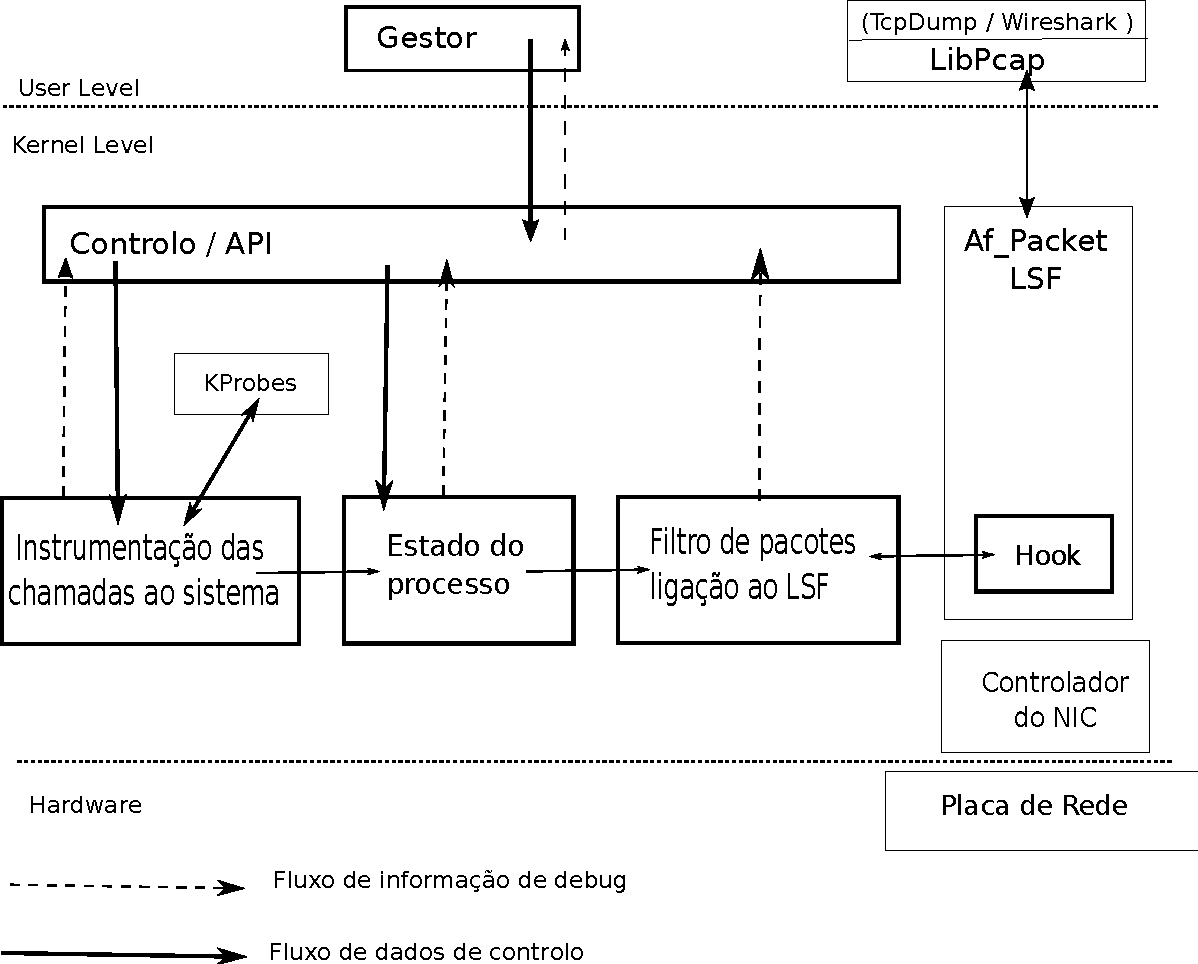
\includegraphics[scale=0.5]{interface.pdf} 
\caption{Arquitectura da solução}
\label{arquitectura}
\end{center}
\end{figure}


Este sistema permite que sejam capturados os pacotes de rede de um processo, sem que exista um conhecimento prévio sobre o(s) protocolo(s) ou portas em utilização. A utilização de um sistema de instrumentação do núcleo foi necessária apenas para monitorizar as chamadas envolvendo \emph{sockets} e qual o processo responsável, permitindo desta forma obter apenas estas chamadas do(s) processo(s) que realmente são monitorizados. De forma a minimizar a redução de desempenho, todo o sistema foi desenvolvido dentro do núcleo do \textit{Linux}, sem alterações nas interfaces já existentes.  Assim, ferramentas de façam uso da biblioteca \textit{LibPcap}, como o programa \textit{TcpDump} ou suas variantes, podem beneficiar desta extensão sem qualquer alteração e sem impacto relevante no seu desempenho.



\subsection*{Instrumentação das chamadas ao sistema de rede}
\label{sub:mon_syscalls}

Um ponto importante deste sistema, constituiu na garantia que todas as interacções desencadeadas por um processo com o exterior fossem detectadas. Para tal, foi necessário recorrer à monitorização das chamadas ao sistema de rede, ou seja, realizar a monitorização ao nível do Kernel, permitindo, assim, minimizar as trocas de contexto. Tirando partido da utilização do sistema de monitorização KProbes (pertencente ao núcleo do Linux), foi possível realizar a monitorização sob um pequeno conjunto de chamadas ao sistema, nomeadamente: sendto, recvfrom, bind, accept, connect e close. Embora o processo que está a executar a chamada ao sistema esteja a ser filtrado, verificou-se que aquando da chamada ao sistema close, ao ser utilizada intensivamente por todo o sistema de ficheiros, esta poderia constituir num ponto onde o sistema iria obter pior desempenho. Desta forma, decidiu-se aplicar a monitorização à função sock\_close, garantindo apenas que os processos que fizessem uso do sistema de transferência de dados, utilizando os métodos da rede, fossem utilizados. Deste modo, foi possível reduzir significativamente o número de eventos de monitorização da chamada ao sistema close.

\subsection*{Filtro de pacotes}
\label{sub:packet_filter}

A função de filtragem aplicada a este sistema assenta no uso de filtros dinâmicos, aos quais permitem efectuar monitorização de rede com ou sem o sistema de filtragem de pacotes definidos no Linux Socket Filter. Deste modo, para minimizar as alterações ao nível da monitorização de rede no Linux, introduziu-se um hook no sistema de rede. Através da utilização deste hook, quando ligado, permite que a monitorização passe pelo sistema dinâmico de filtragem, possibilitando efectuar uma nova monitorização e tirar partido dos benefícios da utilização do Linux Socket Filter.

\subsection*{Estado do processo}
\label{sub:data_repository}

Os portos TCP e UDP em utilização por um dado processo necessitam ser guardados num repositório de dados, para que quando chegue um pacote à interface de rede, este possa ser comparado \td{explicação um pouco mais detalhada}. A estrutura dados escolhida para o efeito, para produzir o repositório pretendido, corresponde a uma árvore \textit{Red and Black}. O uso deste tipo de estrutura permite que o conteúdo da árvore esteja balanceado/equilibrado, obtendo-se um bom compromisso de tempo de acesso à estrutura \textit{versus} quantidade de memória utilizada.

\subsection*{Informação de análise}
\label{sub:data_information}

De forma a poder indicar qual o processo que se deseja monitorizar foram criados três ficheiros. Estes foram criados no sistema de ficheiros virtual \textit{DebugFs}~\cite{DebugFs}.

\subsection{Aplicação Monitorizadora}
\label{sub:monitor_app}
Para poder efectuar os testes de avaliação foi criado uma aplicação em nível utilizador para poder lançar sob seu controlo a aplicação a ser monitorizada.

\section{Avaliação}
\label{sec:evaluation}
O sistema implementado foi avaliado funcionalmente através da utilização de protocolos \textit{ftp}\cite{ftp-proto} e \textit{http} \cite{HypTraPro--HTT}. Para tal, recorreu-se a um conjunto alargado de testes, tendo como objectivo não só observar o seu desempenho, como também, e mais importante, verificar a correcção de todos os pacotes envolvidos nas comunicações. Através destes conjunto de testes, foi possível efectuar a captura dos pacotes resultantes da transferência de um ficheiro, a partir de um servidor ftp ou http. 

De modo a realizar estes testes de desempenho, foram utilizadas duas máquinas ligadas directamente, através da utlização de um cabo Ethernet cruzado. Uma das máquinas ficou responsável pela execução dos serviços \textit{ftp}, \textit{http} e \textit{iperf}.

\subsection{Avaliação Funcional}
A análise funcional foi efectuada por meio de programas simples, que desencadeiam chamadas ao sistema de operação, obtendo-se os dados (portos e endereços) dentro do módulo do núcleo. Estes dados podem ser acedidos através do sistema \textit{debugfs}, onde previamente foi registado um ficheiro para esse efeito. Este ficheiro, quando acedido, contem toda a informação relativa aos portos e endereços em utilização por parte da aplicação monitorizada.
Deste modo, para obter um grau de comparação dos dados produzidos e validar esta análise, foi utilizada a ferramenta \textit{netstat}~\cite{netstat}, na qual indica os dados relativos aos portos e endereços utilizados pelos processos do sistema (esta ferramenta tira partido do sistema de ficheiros virtual \textit{ProcFs} ~\cite{procfskernel} para obter esses dados.

\subsection{Avaliação do desempenho}
Embora exista uma validação funcional do sistema implementado, foram também elaborados diversos testes de desempenho sobre o mesmo. Estes testes focaram-se na recepção ou transmissão de 1GigaByte de dados entre as duas máquinas conectadas directamente por interfaces de rede a 100 Mbit/s.

Na execução destes testes, foram executadas 10 iterações para cada tipo considerado, de modo a obter o valor médio com um desvio padrão aceitável (os resultados obtidos estão descritos nas tabelas \ref{tab:desempenho} e \ref{tab:overhead}).

\begin{table}
\begin{center}

\begin{tabular}{ | c | c | c | c |  }
\hline
Teste & \hspace {0.3cm} Original \hspace {0.3cm}& \hspace {0.2cm} Com TcpDump \hspace {0.2cm} & Com TcpDump e módulo \\
\hline
1GB - FTP & 91.8508	& 1.8500 & 91.8854 \\
1GB - HTTP & 91.6391 & 91.6472 & 91.6674 \\ 
%5GB - HTTP & 457.9506 & 457.9527 & 458.2059 \\
IPerf - 1GB TCP & 91.3790	& 91.2535	& 91.2672 \\
%IPerf - 1GB UDP & 89.7907 & 89.7952 & 90.036 \\
\hline
\hline
1GB HTTP 2 processos & 182.1573 & 188.7156 & 182.0161 \\
\hline
\end{tabular}
\caption{Tempos médios em segundos (s)}
\label{tab:desempenho}
\end{center}
\end{table}

Analisar estes dados .....

\begin{table}
\begin{center}

\begin{tabular}{ | c | c | c | c | }
\hline
Teste & TcpDump com módulo & Variação do TcpDump & \hspace {0.3cm} TcpDump \hspace {0.3cm}\\

\hline
1GB - FTP  & 0.0377 & 0.0385 & -0.0009 \\
1GB - HTTP &  0.0309 & 0.0220 & 0.0088 \\
%5GB - HTTP &  0.0557 & 0.0553 & 0.0005 \\
IPerf - 1GB TCP &  -0.1223 & 0.015 & 0.1373 \\
%IPerf - 1GB UDP & 0.2732 & 0.2682 & 0.0050 \\
\hline
\hline
1GB HTTP 2 processos & -0.0775 & -3.5501 & 3.6003 \\
\hline
\end{tabular}
\caption{Sobrecarga das transferências (valores em percentagem)}
\label{tab:overhead}
\end{center}
\end{table}


analisar estes dados ....

\subsubsection{Desempenho da estrutura de dados}
Para além das avaliações descritas anteriormente, tornou-se essencial analisar o comportamento da estrutura de dados utilizada (também descrita como estrutura de “estado do processo”), de modo a verificar o compromisso entre o desempenho, a versatilidade e o espaço ocupado da mesma, sobre o sistema criado. Assim, para analisar estes pressupostos,foi elaborado um teste recorrendo ao sistema de alta resolução de temporizadores (HRTimer) \cite{hrtimerKernel}, contido no núcleo do sistema de operação.

\begin{table}
\begin{center}

\begin{tabular}{ | c | c |  }
\hline
Teste & \hspace{1cm}Duração\hspace{1cm} \\
\hline
Adicionar 1 elemento & \\
\hline
Adicionar 1024 elementos & \\
\hline

\hline
\end{tabular}
\caption{Tempos em microsegundos}
\label{tab:tree_info}
\end{center}
\end{table}

\subsubsection{Desempenho do Sistema de instrumentação}
Sendo a instrumentação do sistema um ponto fundamental na execução da monitorização de uma aplicação, a análise ao seu comportamento é bastante importante, na medida em que é necessário verificar se a introdução deste tipo de sistemas, irá produziruma elevada penalização sobre o sistema de operação. Tendo em conta que o sistema de instrumentação utilizado corresponde ao \textit{KProbes}, foi fundamental efectuar esses testes, de modo a garantir que tal factor não sucedia, através dos valores indicados em \cite{KProbeKernel}.

\begin{table}
\begin{center}

\begin{tabular}{ | c | c |  }
\hline
Teste & \hspace{1cm}Duração\hspace{1cm} \\
\hline
100 000 000 chamadas & \\
\hline
 & \\
\hline

\hline
\end{tabular}
\caption{Tempos em }
\label{tab:kprobes_info}
\end{center}
\end{table}


\section{Trabalho Relacionado}
\label{sec:related_work}
Trabalhos anteriores tentaram resolver os mesmos problemas mas continuavam a ter número de trocas de contexto.

Um dos trabalhos efectuado por Nuno Farruca~\cite{Farruca:2009,duarte10}, monitorizou os processos por duas vias. Monitorizar o processo através da criação de uma biblioteca que mapeia as funções da biblioteca de C \textit{LibC} e modificando a variável LD\_PRELOAD, de forma a que quando fosse efectuada uma função da biblioteca de C que estivesse mapeada na biblioteca desenvolvida, estas fosse chamada primeiro de forma a obter os parâmetros das funções e assim comunicar à \textit{LibPCap} se os pacotes pertencentes a um determinado porto de um endereço são ou não para capturar. Uma outra forma foi obter os dados dos sockets pertencentes ao processo através do sistema de ficheiros virtual \textit{ProcFs} e executar a filtragem também em nível utilizador dos pacotes que chegam à interface capturadas através da \textit{LibPcap}.

O trabalho~\cite{1688981} com o título \textit{Application-specific packet capturing using kernel probes}, efectuou uma monitorização, utilizando o sistema de instrumentação \textit{KProbes}, das funções de transmissão e recepção de dados dentro do núcleo do sistema. Desta forma é possível monitorizar os dados de um processo. Os dados recolhidos são analisados com o intuito de perceber se determinada porta e endereço são conhecidos e caso não sejam é adicionada a informação a uma tabela de dispersão utilizada para efectuar um novo filtro. O pacote capturado  é atrasado e re-injectado e forma a poder ser capturado pela biblioteca \textit{LibPCap} através do novo filtro.

\section{Conclusões}
\label{sec:conclusions}


\bibliographystyle{plain}
\bibliography{references}

\end{document}
